\documentclass{article} % For LaTeX2e
\usepackage{nips13submit_e,times}
\usepackage{hyperref}
\usepackage{url}
\usepackage{graphicx}
%\documentstyle[nips13submit_09,times,art10]{article} % For LaTeX 2.09


\title{  Extracting and Aggregating Aspect-Level Sentiment from Product Reviews  }


\author{
Desmond C. Ong, Shane Soh, Matthew Long \\
Stanford University \\
\texttt{\{dco, shanesoh, mlong14\}@stanford.edu}
%Matthew Long \\
%Stanford University\\
%\texttt{mlong14} \\
%\And
%Desmond C. Ong \\
%%Psychology \\
%Stanford University \\
%\texttt{dco} \\
%\And
%Shane Soh \\
%%Affiliation \\
%Stanford University \\
%\texttt{shanesoh} \\
}

% The \author macro works with any number of authors. There are two commands
% used to separate the names and addresses of multiple authors: \And and \AND.
%
% Using \And between authors leaves it to \LaTeX{} to determine where to break
% the lines. Using \AND forces a linebreak at that point. So, if \LaTeX{}
% puts 3 of 4 authors names on the first line, and the last on the second
% line, try using \AND instead of \And before the third author name.

\newcommand{\fix}{\marginpar{FIX}}
\newcommand{\new}{\marginpar{NEW}}

\nipsfinalcopy % Uncomment for camera-ready version

\begin{document}


\maketitle

\begin{abstract}
Previous work in \textit{aspect-level sentiment analysis}---identifying the sentiment associated with products and their individual attributes, like battery life---have mostly been formulated as supervised learning problems, requiring known labels of both the relevant aspects and their sentiment. Such labeled datasets are rare, and often very small. Here we propose a scalable hybrid method where we first generate aspects from natural language text via unsupervised clustering of word vector representations, and secondly extract aspect-level sentiment. We then proceed to summarize these aspect-level sentiment within and across reviews and provide visualizations to aid consumers.
\end{abstract}

\section{Introduction}

In today's e-commercialized society, the consumer not only has access to online stores through which she might purchase anything she desires, but she also has unprecedented access to a deluge of information---most notably, product reviews written by other consumers---with which she can make her decision. Unfortunately, sifting through hundreds of reviews across tens of different websites to acquire specific information about the product and its important attributes (e.g. \textit{battery life}, \textit{screen size}, or \textit{weight} for electronics) is a time-consuming chore. It is difficult to automatically summarize this information, especially because of the heterogeneity of attributes across different product categories. Because of this, there has been much recent research tackling the two separate but interconnected components of this problem: (1) automatic discovery of aspects, and (2) aspect-specific sentiment analysis.

Within the context of a product review, the first component, \textit{aspect discovery}, involves identifying individual ``aspects" (which could be the product itself, or features/attributes of the product). This is made more difficult by the fact that relevant aspects might differ across similar products. For example, for a given electronic item such as a mobile phone, relevant aspects could be the battery life, screen size, weight, cost, and more. Not all these aspects are relevant across other electronic items: for a computer, weight might not be an issue, and screen size might be moot for headphones. 

The second component, \textit{aspect-specific sentiment analysis} involves subsequently identifying the sentiment---positive, neutral, or negative judgments---associated with aspects [1-6]. This essentially boils down to solving $n$ separate sentiment analysis problems per document, where $n$ is the number of aspects, and doing proper assignment of sentiment to aspects. Needless to say, this is a challenging task that is starting to receive much attention by researchers in the past few years.

One of the challenges is the lack of large labeled datasets with which to train supervised models. In this paper, we propose a scalable hybrid method that is almost entirely unsupervised, that enables learning of aspect-specific sentiment on large datasets.





\section{Related work}

\textbf{Aspect Discovery}: Previous methods have used graphical models to attempt to extract latent sentiment.[1-3] use Latent Dirichlet Allocation, while [4] uses a Conditional Random Field model to model latent aspects. In particular, most of these methods have a generative model where there is a latent aspect (drawn from a mix of ``global" and ``local" topics [1-2], or latent to each sentence [3])

We propose using similar unsupervised methods to generate candidate aspects via semantic word vector representations. 

In this paper, we propose extending recent successful advances in deep learning [6-7] to address this problem. In particular, we seek to improve and extend the work in [6], who used deep learning architectures like the Recursive Neural Tensor Network (RNTN) to extract aspect and sentiment in a single step. Unfortunately, supervised methods (e.g. [5-7]) that require labeled aspects-sentiment pairs for training are unscalable, and a better approach would be to automatically identify relevant aspects for each product (which, e.g. [1-3] try to do via topic modeling). 




\section{Approach}

Our proposed workflow can be divided into two main parts: (unsupervised) {\bf Aspect Discovery} and {\bf Aspect-Specific Sentiment Extraction}. See Fig. \ref{workflow} for an illustration.


\begin{figure}[ht]
\begin{center}
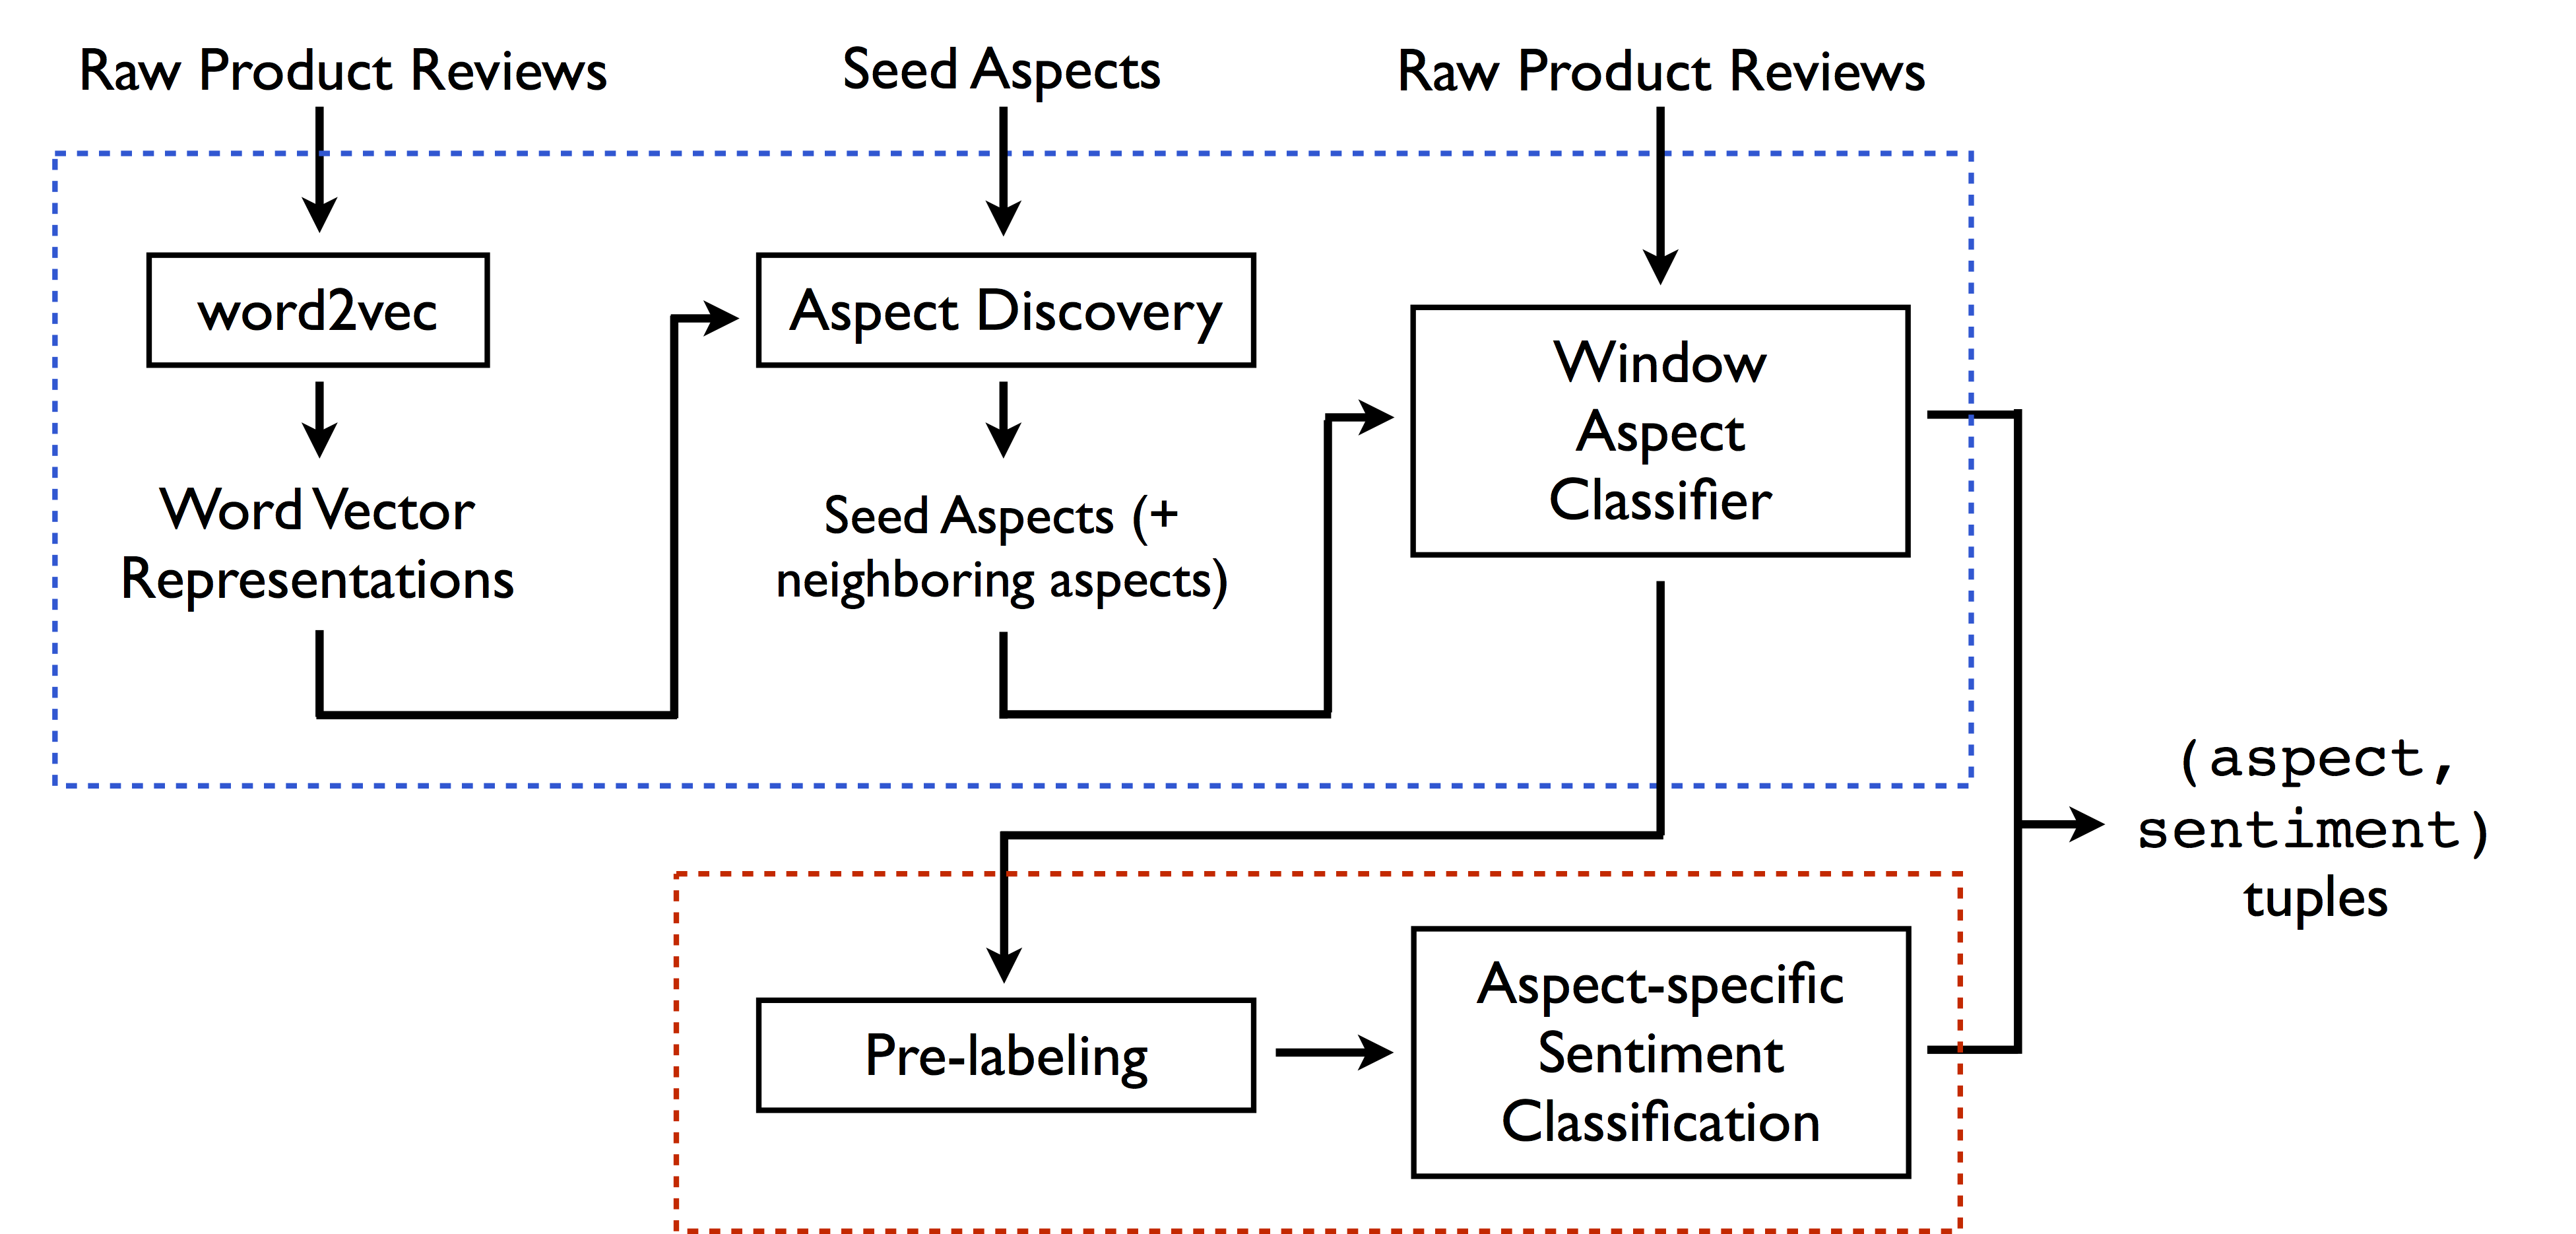
\includegraphics[width=.85\columnwidth]{workflow.png}
\end{center}
\caption{Proposed Workflow. We first use a word2vec representation to discover new aspects, and to identify aspects in the data. Next, we classify the sentiment of the surrounding context. This generates a labeled dataset on which we train a deep CNN to perform aspect-specific sentiment extraction.}% Except for the Sentiment Labeling and Visualization processes, every other process involves deep learning.}
\label{workflow}
\end{figure}


\subsection{Aspect Discovery}

The first part of our workflow involves an unsupervised approach to generating aspects. Our intuition is that we can use similarity in a high dimensional word vector embedding space to find closely related groups of words. Words may be grouped by syntactic class (e.g. nouns), by similarity in context (e.g. ``X is great"), or by other words that they co-occur with, etc, and we hoped to use this similarity to automatically discover new aspects from a starting seed list.

\subsubsection{Preprocessing.} We tokenized our corpus using NLTK's punkt tokenizer [9] for sentence splitting. We then removed all non-alphanumerical characters and replaced all digits with \texttt{DG}. Finally, we performed collocation detection to detect common bigrams. We run word2vec (CBOW, Skipgram) to obtain a word vector representation of the data (varying hyper parameters like window size). 

\subsubsection{Seed words and discovery.} We handcrafted a small set of 63 seed attributes from reading a random sample of product reviews. We then used these seed aspects and our word2vec model representation to discover more aspects via closest cosine similarity.

\subsubsection{NER Model?}

NER Model architecture


\subsection{Aspect-Specific Sentiment Extraction}

The second half of our workflow involved sentiment analysis given identified aspects. Our intuition for this part stems from locality: if there are multiple sentiment and multiple aspect words within a sentence, then a good ``heuristic" would be that sentiment words closer to a particular aspect should be attributed to that aspect. Hence, models should be able to make use of local context to help in sentiment attribution.

We decided upon a Convolutional Neural Network (CNN) Model based after Kim [10], who reported excellent results in sentence classification on many tasks, including sentiment analysis. We model our architecture, shown in Figure \ref{architecture} on [10].


%An additional step would be to label all unigrams with a sentiment analysis lexicon (Bing Liu's sentiment lexicon) or the Sentiment pipeline in CoreNLP [7]. With the aspect-labels from the previous part, we would have a dataset labeled with aspect and (unigram-) sentiment. Next, we build off and improve on the model in [6]: we will use a RNTN or improved architecture to extract (aspect, aspect-specific sentiment) tuples from the data. Finally, we will have a summarization of aspect-related sentiment via visualization of our output, in terms of a word cloud of important aspects (e.g., sized by word frequency and colored by sentiment). 




\begin{figure}[ht]
\begin{center}
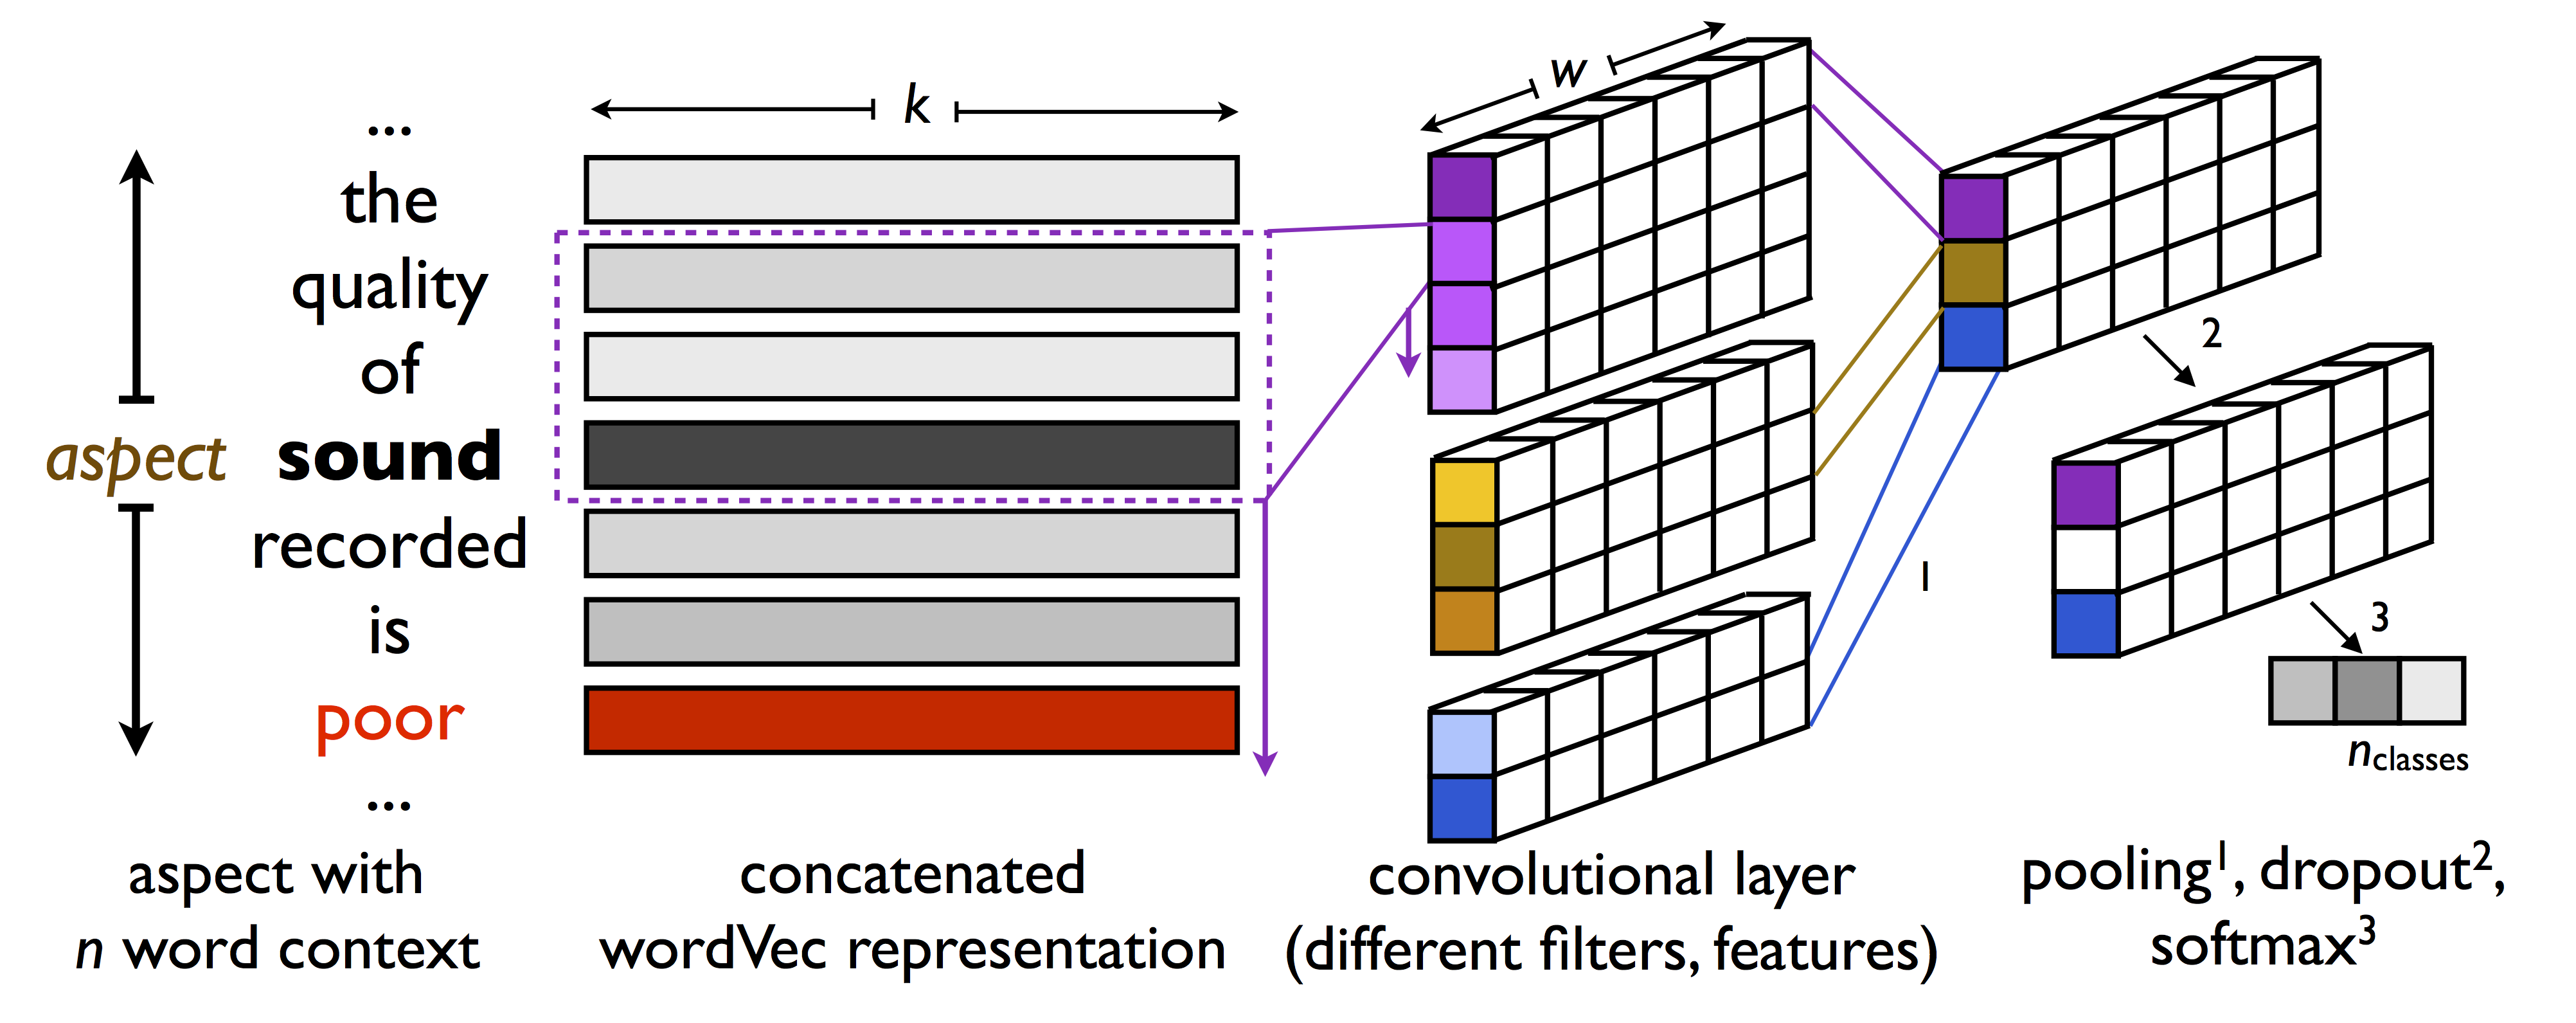
\includegraphics[width=\columnwidth]{model_architecture.png}
\end{center}
\caption{CNN Model Architecture, modeled after Kim [10]. The input is an $n$ word context}
\label{architecture}
\end{figure}


\section{Experimental Results} 

\textbf{Dataset.} The dataset that we used consists of 7.6 million reviews of electronic products from Amazon.com [8]. These reviews comprise 39.4 million sentences. Each review is only labeled with the document-level 5 star rating, which we did not end up using as it was too coarse. We focused our attention only on the raw natural language text, which is unlabeled.


\subsection{Aspect Discovery Model Training} 

We trained three different word2vec models. The most successful model was trained using the CBOW (continuous bag-of-words) model with a window size of 10 and feature dimension size of 300. We also ignored all words with total frequency count below 40 (this helped to remove many misspellings). We determined the performance of each model by querying the model with various aspects common to electronic products (e.g. "portability", "screen quality", etc).

\subsection{word2vec Results}

\begin{figure}[ht]
\begin{center}
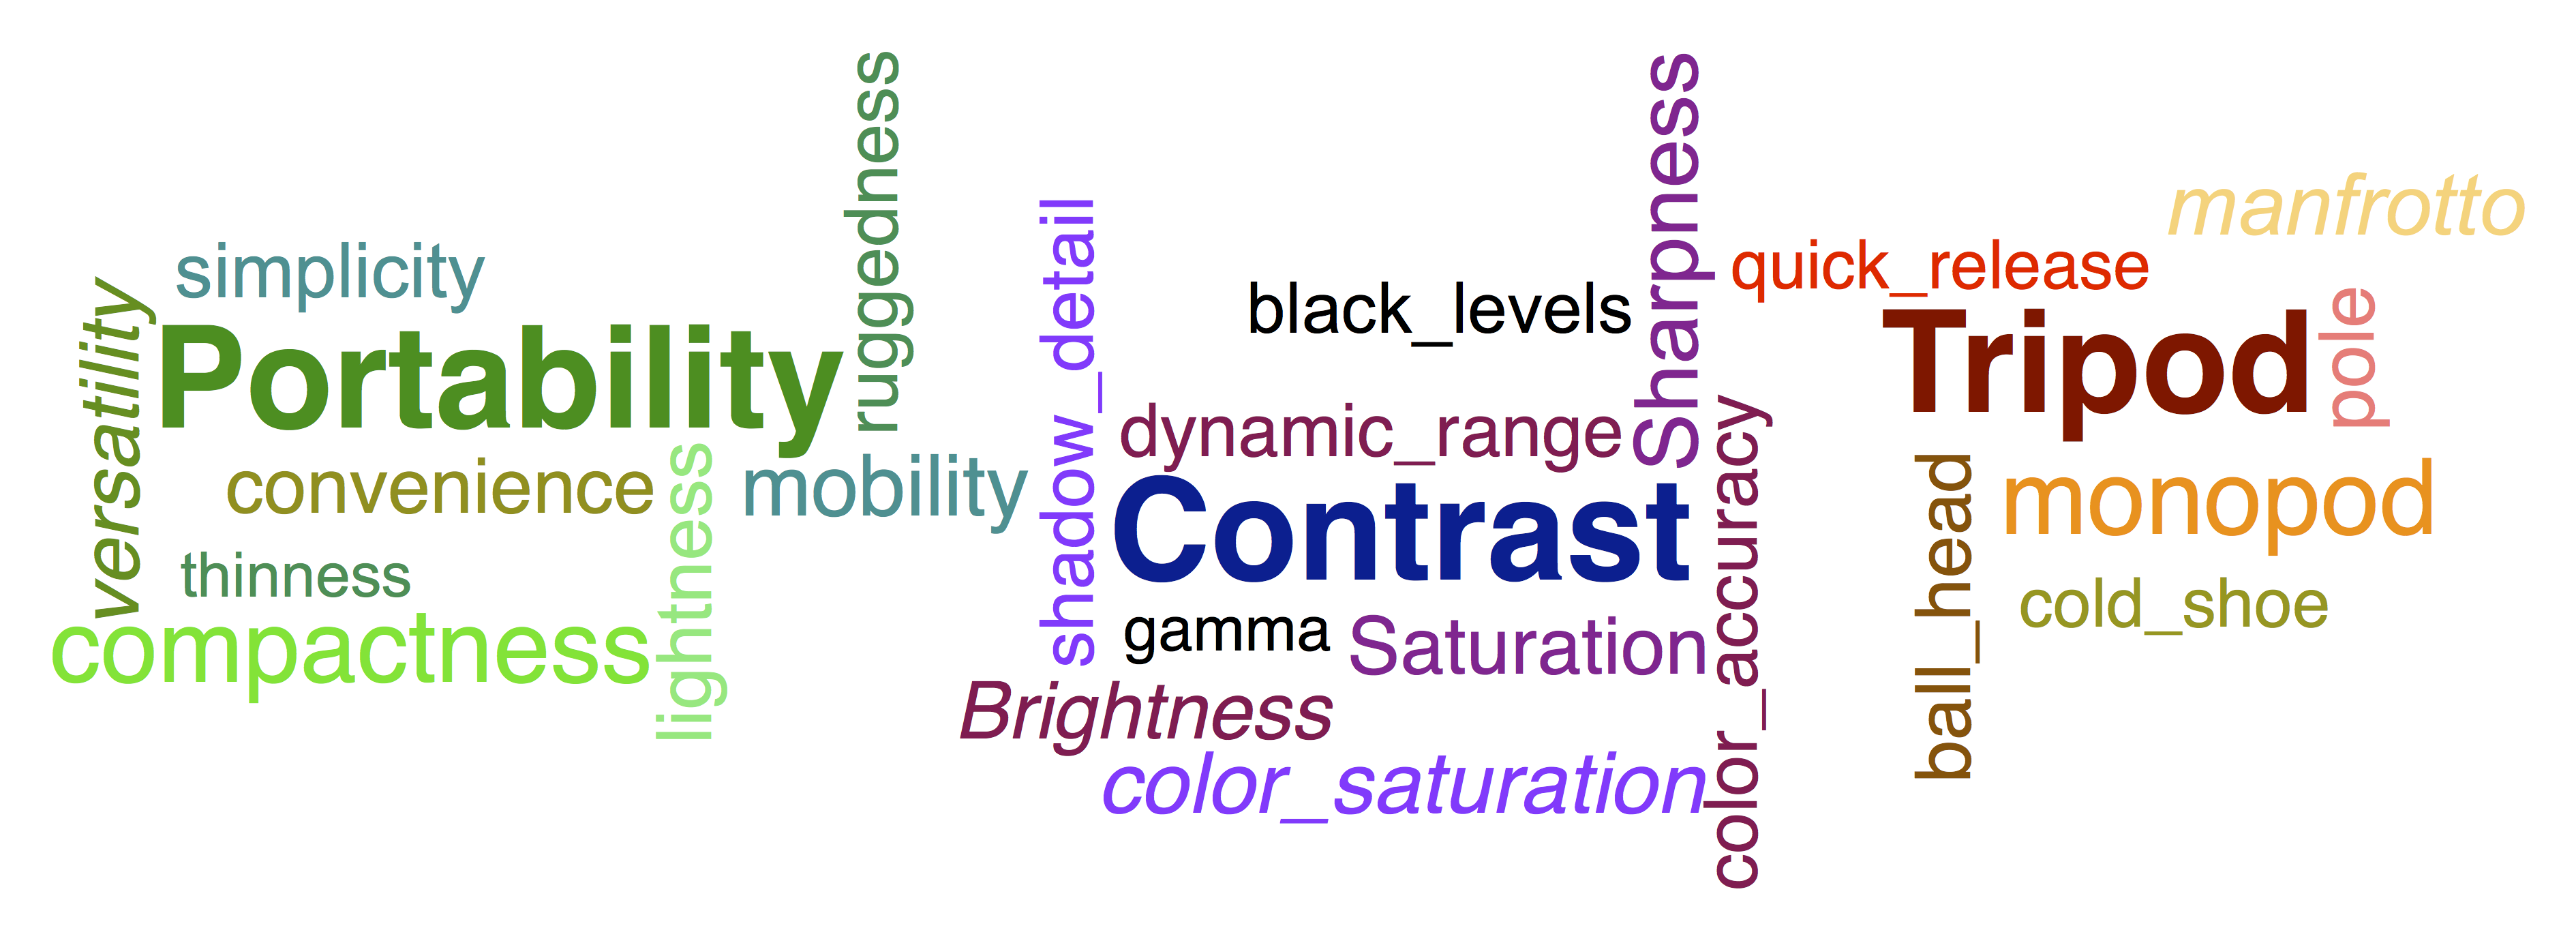
\includegraphics[width=\columnwidth]{Aspects_long.png}
\end{center}
\caption{Aspects Discovery. Word clouds generated by seeding \texttt{portability} (left), \texttt{contrast} (middle), and \texttt{tripod} (right). Words are sized according to cosine similarity with the seed word.}
\label{aspectFig}
\end{figure}

We queried our word2vec model and returned the top-$n$ results based on cosine similarity of the word vectors, as illustrated in Figure \ref{aspectFig}. We found that $n=5$ is a good number that maintains the quality of aspects while allowing a good discovery ratio (Fig. \ref{aspectFig} was made with more than 5 closest results).

As shown in Fig. \ref{aspectFig}, words like \texttt{portability} returned many synonyms as well as product aspects that are related to it (e.g. \texttt{ruggedness} and \texttt{simplicity}). Our model is also capable of returning aspects that are specific and unique to the product category it is trained on. In this case of electronic products, a query like \texttt{contrast} returned words like \texttt{shadow\_detail}, \texttt{dynamic\_range}, \texttt{black\_levels} and \texttt{gamma}, which are aspects specific to devices like monitor displays and cameras. Finally, the query \texttt{tripod} returned various aspects of camera tripods, many of them being features that are non-obvious to the layperson. For instance, \texttt{ball\_head} refers to a type of ball-shaped tripod head that allows free-pivoting along two rotational axes (as opposed to Cartesian axes), and \texttt{quick\_release} refers to tripod mounts that come with a quick-release plate. Many of these queries would otherwise perform poorly if performed on lexical databases like WordNet.


\subsubsection{NER Model?}

NER Model results


\subsection{Aspect-Specific Sentiment Extraction}


% Socher's model (down the rows) vs. human labels. So there were 16 instances that human says 2 and model says 1.
%							True Labels
%			1		2		3		4		5
%1			9		16		5		10		4		44
%2			168		495		404		180		124		1371
%3			230		590		1528		488		303		3139
%4			21		70		494		490		281		1356
%5			0		0		9		65		16		90
%			428		1171		2440		1233		728		6000

As our data was entirely unlabeled, we initially attempted to bootstrap training of our CNN model using labels obtained from other trained sentiment-analysis models. We felt, however, that this would be a major limitation, as we would have labels of uncertain quality and accuracy (we discuss this more below). Hence, to properly evaluate our approach, we decided to hand label some data and use a semi-supervised approach to build a larger model. Unfortunately we did not complete our ambitious, semi-supervised goal. Below, we report our quantitative evaluation.

Using the first model developed above, we extracted 6,000 examples which consisted of an identified aspect, surrounded by a context of 5 words on either side. We padded these phrases with sentence start and end tags, and with zero vectors. Next, we hand-labeled these 6,000 examples on a 5 point scale, corresponding to Very Negative, Negative, Neutral, Positive, and Very Positive. 

We trained our CNN on this dataset, using a 10-fold cross validation strategy and reporting on a 10\% test set. The results are given in Table \ref{ModelResultsTable}. The CNN, with <hyperparameters FIXME> achieved an accuracy of FIXME on the 5 class classification, and, if we combined the classes to a coarser, 3 class (Positve, Neutral, Negative) task, achieved an accuracy of FIXME.

Next, we sought to test our original idea of ``bootstrapping" labels using existing pre-trained models. On the one hand, there are models that are trained on much larger amounts of labeled data, sometimes even down to the unigram level, e.g. Socher et al [7]. On the other hand, these models are often trained on other domains ([7] was trained on movie reviews), and it is still an open question as to the degree of cross-domain transfer. To test this, we ran the Stanford CoreNLP Sentiment Annotator [7], which also outputs 5 classes, on our 6,000 labeled examples. The 5-class accuracy was 42.3\%, while the coarser 3 class accuracy was 51.1\%.

We must be upfront and say that our point of performing this was \textbf{not} to use [7] as a baseline for comparison: indeed, it was trained out of domain, while our model was trained within domain. (Note, however, that [7] reported a test accuracy within their own dataset of 45.7\% on a 5 class task, and 85.4\% on a 2 class (positive/negative) task, so at least the first result is comparable to what we found.) Rather, we performed this analysis to gauge the upper limit on our model's reliability if it were only trained using labels obtained from out-of-domain pre-trained models (which, this analysis shows, has ~50\% accuracy with respect to a labeled gold standard on a 5 class task).

\begin{table}[t]
\begin{center}
\begin{tabular}{lll}
\multicolumn{1}{c}{\bf Sentiment Model}  &\multicolumn{1}{c}{\bf 3-class Accuracy} &\multicolumn{1}{c}{\bf 5-class Accuracy} \\ \hline
 Our CNN\textsuperscript{1} & 79.4\% \textbf{(FIXME)} & 64\% \textbf{(FIXME)} \\
 Pre-trained out-of-domain RNTN [7]\textsuperscript{2}       & 51.1\% & 42.3\% \\
\end{tabular}
\end{center}
\caption{Accuracies for different models. \textsuperscript{1} was trained }
\label{ModelResultsTable}
\end{table}



\subsection{Qualitative evaluation of sentiment}

\textbf{Evaluation}: We will construct word cloud visualizations color coded to express sentiment. We will also perform comparisons with ``expert review" sites like CNET and DPReview (e.g. DPReview specifically rates digital cameras along certain chosen dimensions).


compare with google product reviews / cnet reviews

Error analysis (but actually we don't know if our model fails on these, we don't really have item level aspect

One common aspect that our method identified was \texttt{speed}, in terms of computer or processing speed. This also led to the discovery of \texttt{speed\_limit}, in the context of GPS reviews where GPSes are programmed with the speed limit of roads. While it might be arguable that knowing the road speed limit is a relevant aspect of a GPS, this highlighted the fact that our model might not be able to capture instances where words have different meanings in different contexts.

One problem with aspect-specific sentiment analysis in product reviews is that many reviewers discuss how the new product fares in relation to an older, similar product they owned. For example, phrases like ``my old laptop was better" seems semantically positive, but reflects negative sentiment with respect to the product being discussed. We hoped that increasing the context window would allow the model to pick up comparative words (especially that interacts with which is the subject and object of comparison).



word cloud
size = frequency of aspect over several reviews
color = valence

\section{Discussion}

Even our mediocre labeling (6000 examples) was comparable with many existing datasets out there (e.g. the Beer Advocate dataset and Camera Review dataset reported in [6] had about 8,000 and 4,000 labeled sentences respectively).

\section{Conclusion}

conclusion

cost efficient, time consuming






\subsubsection*{Acknowledgments}

We would like to acknowledge funding for computing resources provided by the Deep Social Learning Lab at Stanford.

\subsubsection*{References} % chronological. Use APA

\small{

[1] Titov, I., \& McDonald, R. T. (2008). A Joint Model of Text and Aspect Ratings for Sentiment Summarization. In {\it ACL} (Vol. 8, pp. 308-316).

[2] Brody, S., \& Elhadad, N. (2010). An unsupervised aspect-sentiment model for online reviews. In {\it Human Language Technologies: The 2010 Annual Conference of the North American Chapter of the Association for Computational Linguistics} (pp. 804-812). Association for Computational Linguistics.

[3] Jo, Y., \& Oh, A. H. (2011). Aspect and sentiment unification model for online review analysis. In Proceedings of the fourth ACM international conference on Web search and data mining (pp. 815-824). ACM.


[4] Engonopoulos, N., Lazaridou, A., Paliouras, G., \& Chandrinos, K. (2011). ELS: a word-level method for entity-level sentiment analysis. In {\it Proceedings of the International Conference on Web Intelligence, Mining and Semantics}


[5] Moilanen, K., \& Pulman, S. (2009). Multi-entity Sentiment Scoring. In {\it Recent Advances in NLP} (pp. 258-263).


[6] Lakkaraju, H., Socher, R, \& Manning, C. (2014). Aspect Specific Sentiment Analysis using Hierarchical Deep Learning. {\it NIPS Workshop on Deep Learning and Representation Learning}

[7] Socher, R., Perelygin, A., Wu, J. Y., Chuang, J., Manning, C. D., Ng, A. Y., \& Potts, C. (2013). Recursive deep models for semantic compositionality over a sentiment treebank. In {\it Proceedings of the conference on Empirical Methods in Natural Language Processing (EMNLP)} (Vol. 1631, p. 1642).


%[8] Ghose, A., \& Ipeirotis, P. G. (2007). Designing novel review ranking systems: predicting the usefulness and impact of reviews. In {\it Proceedings of the Ninth international conference on Electronic commerce} (pp. 303-310). ACM.

%[9] Chen, P. Y., Dhanasobhon, S., \& Smith, M. D. (2008). All reviews are not created equal: The disaggregate impact of reviews and reviewers at Amazon.com. Available at SSRN: http://ssrn.com/abstract=918083 

%[10] Dai, W., Jin, G. Z., Lee, J., \& Luca, M. (2012). Optimal aggregation of consumer ratings: an application to Yelp.com (No. w18567). National Bureau of Economic Research. 


[8] McAuley, J., Targett, C., Shi, J., \& van den Hengel, A. (2015). Image-based recommendations on styles and substitutes. {\it ACM Special Interest Group on Information Retrieval (SIGIR)}

[9] Bird, Steven, Loper, E. and Klein, E. (2009). Natural Language Processing with Python. O'Reilly Media Inc.

[10] Kim, Y. (2014). Convolutional neural networks for sentence classification. EMNLP.

%% this paper isn't that relevant. it's an evaluation system.
%[2] Ward, C. B., Choi, Y., Skiena, S., \& Xavier, E. C. (2011). Empath: A framework for evaluating entity-level sentiment analysis. In {\it Emerging Technologies for a Smarter World (CEWIT), 2011 8th International Conference \& Expo}. (pp. 1-6). IEEE.


%
%Wang, H., Lu, Y., & Zhai, C. (2010, July). Latent aspect rating analysis on review text data: a rating regression approach. In Proceedings of the 16th ACM SIGKDD international conference on Knowledge discovery and data mining (pp. 783-792). ACM.
%
%Yatani, K., Novati, M., Trusty, A., & Truong, K. N. (2011, May). Review spotlight: a user interface for summarizing user-generated reviews using adjective-noun word pairs. In Proceedings of the SIGCHI Conference on Human Factors in Computing Systems (pp. 1541-1550). ACM.



}

\end{document}
